\documentclass[11pt]{article}

\usepackage{booktabs}
\usepackage{tabularx}
\usepackage{makecell}
\usepackage{enumitem}
\usepackage{microtype}
\usepackage{subcaption}
\usepackage{listings}
\usepackage{amsmath}
\usepackage{amssymb}
\usepackage{graphicx}
\usepackage[letterpaper,margin=1in,includefoot]{geometry}
\usepackage[hidelinks]{hyperref}
\usepackage[numbers]{natbib}
\usepackage{fancyhdr}

\pagestyle{fancy}
\fancyhf{}
\fancyfoot[R]{\thepage}
\renewcommand{\headrulewidth}{0pt}
\renewcommand{\footrulewidth}{0pt}

\newcommand{\Description}[1]{}

\graphicspath{{../../experiments/figures/}}

\setlength{\textfloatsep}{12pt plus 2pt minus 2pt}
\setlength{\floatsep}{10pt plus 2pt minus 2pt}
\setlength{\intextsep}{10pt plus 2pt minus 2pt}
\newcolumntype{Y}{>{\raggedright\arraybackslash}X}

\newcommand{\dataset}{\mathcal{D}}
\newcommand{\retained}{\mathcal{D}'}
\newcommand{\queries}{\mathcal{Q}}
\newcommand{\budget}{B}
\newcommand{\cosim}{\operatorname{cos}}
\newcommand{\argmax}{\operatorname*{arg\,max}}

\title{Query-Aware Photo Selection for Data Reduction}

\author{Luca Foresti}
\date{June 25, 2026}

\begin{document}
\hypersetup{pageanchor=false}
\pagenumbering{gobble}
\begin{titlepage}
  \thispagestyle{empty}
  \centering
  \vspace*{0.18\textheight}
  {\LARGE\bfseries Query-Aware Photo Selection for Data Reduction\par}
  \vspace{2.5cm}
  {\large Author\par}
  \vspace{0.25cm}
  {\Large Luca Foresti\par}
  \vspace{2.0cm}
  {\large Report created\par}
  \vspace{0.25cm}
  {\Large June 25, 2026\par}
  \vfill
  {\large Roma Tre University\par}
  \vspace{0.2cm}
  {\large Matricola: 565562\par}
\end{titlepage}

\clearpage
\hypersetup{pageanchor=true}
\pagenumbering{arabic}
\setcounter{page}{1}

\begin{abstract}
Smartphone photo collections grow quickly, but storage and search quality impose practical limits on how many images can be retained. This project studies query-aware photo selection: given photo embeddings and a historical query log, select a budgeted subset that preserves the usefulness of past search results. I implement four methods required by the assignment: exhaustive cosine-based selection, IndepDF with Jaccard-style scoring, exact Shapley-value ranking, and a proposed query-frequency-weighted greedy facility-location method. The implementation includes shared loading, validation, utility, experiment, and plotting code. Experiments on a private dataset of 41,620 photos, 2,048-dimensional embeddings, and 443 query rows show the expected trade-off: exact methods are useful tiny-scale references but infeasible on the full collection, IndepDF is fastest and lightest, and Method D gives the strongest scalable cosine-proxy utility while using more runtime and memory. The repository provides reproducible configs, saved results, generated figures, tests, and lint checks.
\end{abstract}

\noindent\textbf{Keywords:} data reduction, query logs, photo selection, submodular coverage, facility location

\section{Introduction}

Global data production keeps increasing while personal devices still face concrete limits: storage, processing time, energy use, and the human cost of searching through large collections. The practical example in this assignment is a smartphone photo library. The phone is running out of space, so only a subset of photos can be kept. A naive deletion policy may save storage but damage future search quality, especially if deleted photos were historically useful answers to past queries.

The project problem is therefore to select retained photos under a fixed budget while preserving the utility of historical search results. Each photo is represented by an embedding vector, and the query log records which photo identifiers were returned by previous searches. Because the original query operators are not available, the implementation evaluates retained subsets through proxy utilities derived from the historical query results and photo embeddings.

This work follows the assignment framing~\cite{velegrakis2026practical} and the stochastic data-forgetting perspective of Rico, Siebes, and Velegrakis~\cite{rico2026stochastic}. It makes three contributions. First, it implements the three required baselines: Method A, Method B, and Method C. Second, it introduces Method D, a query-frequency-weighted greedy facility-location strategy that combines workload awareness with embedding coverage. Third, it benchmarks all methods where feasible, comparing utility, runtime, memory, scalability, and theoretical complexity in a reproducible Python repository.

\subsection{Assignment Interpretation}

The practical assignment gives photo embeddings and a historical query log, but it does not provide the original query operators. This means that the implementation cannot literally re-run a search over a reduced collection. I interpret the query log as empirical evidence of the user's information needs. If a photo appeared often in historical results, deleting it or failing to keep a semantically close representative is more likely to hurt future perceived quality.

This interpretation leads to two complementary metrics: membership utility for direct historical presence, used by Method B, and replacement utility for embedding-similar representatives, used by Methods A, C, and D. The report keeps both metrics separate because the methods optimize different signals.

\subsection{Repository Scope}

The repository is deliberately small and reproducible. It contains data validation, method implementations, experiment scripts, saved result tables, diagnostic JSON files, generated figures, and tests. It does not commit the raw private dataset. Stretch baselines such as random selection, clustering medoids, or Monte Carlo Shapley approximation were not covered.

\section{Background}

The lecture frames data reduction as the choice to retain a smaller dataset that preserves utility under a constraint. This is broader than file compression. Selective storage, coresets, sketches, summarization, redundancy removal, and deletion all reduce data, but they differ in what downstream behavior they preserve. The photo-selection assignment is closest to deletion with workload awareness: the system must decide which original items remain available, and the decision should be guided by past queries.

Workload-aware deletion is especially relevant for personal devices. A photo that has never appeared in historical search results may be less important for search quality than a visually central photo that appeared many times. However, popularity alone is not enough. If five near-duplicate photos all appeared in query logs, keeping all five may waste budget; a single representative can cover that region of embedding space. This is the motivation for combining query frequency with representativeness.

Submodular coverage objectives provide a useful design principle. A set function is submodular when each new item has diminishing marginal value as the selected set grows. Coverage and facility-location objectives often have this property because once an item or region is represented, adding another similar representative helps less. Greedy algorithms are attractive in this setting: they are not exact, but they are simple, scalable, and aligned with the underlying diminishing-returns structure.

Shapley values provide a contrasting view. Rather than searching for a set directly, they assign value to individual data items by averaging marginal contributions over all possible coalitions. This is principled and fair in a game-theoretic sense, but the exact computation is exponential. In this project, Shapley values are therefore best understood as a tiny-scale diagnostic baseline rather than a practical method for the full photo collection.

\section{Problem Formalization}

Let $\dataset$ be the full photo collection. Each photo $d \in \dataset$ is represented as an embedding vector in $\mathbb{R}^{n}$; in the local dataset, $n=2048$. The file \texttt{photos.csv} contains one vector per row. The query log \texttt{queries.csv} contains one historical query result per row, represented as a variable-length list of photo identifiers.

The goal is to choose a retained subset $\retained \subseteq \dataset$ with $|\retained| \leq \budget$, where $\budget$ is the maximum number of photos that can be kept. The ideal objective is to maximize expected query utility:
\begin{equation}
  \dataset^{*} =
  \argmax_{\retained \subseteq \dataset,\ |\retained| \leq \budget}
  \mathbb{E}_{q \sim \queries}\left[S(q(\dataset), q(\retained))\right].
  \label{eq:main-objective}
\end{equation}

Only historical result identifiers are available. The original search functions are not. The implementation therefore uses retained photos as representatives. Each original result photo is matched to its closest retained photo:
\begin{equation}
  S(q(\dataset), \retained)
  =
  \frac{1}{|q(\dataset)|}
  \sum_{d \in q(\dataset)}
  \max_{s \in \retained} \cosim(d, s).
  \label{eq:cosine-proxy}
\end{equation}

Method B uses query-membership IndepDF scores. Each query contributes one over its result length to each returned photo, and these per-query masses are averaged over the query log. The experiment layer records both cosine-proxy utility and Jaccard/precision utility for cross-method comparison. This is important because the methods optimize slightly different proxies: Methods A, C, and D are embedding-aware, while Method B is primarily membership-frequency based.

The data-loading layer normalizes query photo identifiers once, validates bounds and malformed rows, deduplicates per-query IDs, and reports diagnostics. The assignment defines a photo ID by its line in \texttt{photos.csv}; for example, ID 73 is the vector on line 73. The final raw-data experiments therefore use one-based query IDs explicitly. The loader still supports zero-based and automatic modes for tests and reuse, but the canonical result metadata records \texttt{id\_base\_requested=one} and \texttt{id\_base\_resolved=one}.

\subsection{Data Contract}

The photo loader expects a rectangular numeric CSV with no header. Rows with missing values, non-numeric values, unequal embedding dimensions, or zero vectors are rejected or reported according to the validation path. The query loader expects one result set per row and supports variable-length rows. Within a query row, duplicate photo IDs are deduplicated before scoring so that a repeated identifier does not artificially increase a photo's importance.

This separation matters for correctness: all ID normalization is performed before methods run. The methods receive normalized NumPy arrays and do not reinterpret whether IDs are zero-based or one-based. That design prevents a subtle class of bugs where different algorithms silently evaluate different photo identities.

The local validation result gives a useful sanity check on the private data: 41,620 photos, 2,048 embedding dimensions, and 443 query rows. The query log contains 10,937 distinct queried targets after normalization, which is the set that receives positive weight in Method D's full-data run. This means the proposed method evaluates coverage over a much smaller weighted target set than the full matrix of all photos, while still allowing any photo to be selected as a representative.

\subsection{Utility Metrics}

The primary cross-method metric in the report is cosine-proxy utility, because it reflects embedding-level replacement quality and is the objective optimized by Methods A, C, and D. Jaccard/precision utility is recorded as a secondary metric because it is aligned with IndepDF's query-membership view. The experimental result schema stores both metrics for every successful run, plus runtime, peak measured memory, selected normalized IDs, selected original IDs, train and evaluation query counts, evaluation scope, status, message, diagnostics path, config path, Python version, hardware notes, and git metadata.

There are two consequences of this design. First, a method can look good under one metric and less good under another. The frequency-only Method D ablation is the clearest example: it preserves historically frequent memberships but does not cover embedding space as well. Second, the report does not claim that cosine-proxy utility is the true user utility. It is a reproducible proxy that makes the assignment executable with the available files.

\section{Methodology}

All methods expose a shared selection interface returning selected IDs, utility, runtime, peak memory, status, message, and diagnostics. Budgets and exact-method limits are validated before execution. Deterministic lower-ID tie-breaking keeps repeated runs reproducible.

\subsection{Shared Implementation Layer}

The implementation is organized as a Python package under the \texttt{src/} tree. The shared data layer reads and validates CSV files. The similarity layer implements safe cosine operations, including zero-vector handling. The utility layer implements cosine-proxy utility, Jaccard/precision utility, and IndepDF scores. The evaluation layer records timing, measured peak memory, deterministic tie-breaking, status values, and CSV/JSON-friendly result serialization.

This shared layer keeps the method comparison fair. Each method uses the same normalized photo matrix and query list, the same budget validation, and the same evaluation utilities. The experiment runner expands YAML configs into deterministic runs, writes one tidy CSV row per run, and stores method-specific details in diagnostics JSON files.

\subsection{Diagnostics and Status Handling}

Every method can return \texttt{success}, \texttt{skipped}, \texttt{timeout}, or \texttt{error}. Exact Method A and exact Method C use \texttt{skipped} to document infeasible runs without crashing the experiment batch. The skip message and diagnostics explain the configured limit and candidate scale. This is preferable to omitting the run: the report can then show that full-data exact methods were attempted in a controlled way and rejected for theoretical reasons.

Diagnostics also make Method D auditable. The full local Method D run records 10,937 weighted targets, an effective candidate chunk size of 766, a 64 MB facility-similarity limit, and \texttt{float64} numeric math. These values explain why the method can run on the full dataset without allocating a dense all-pairs similarity matrix.

\subsection{Method A: Exact Cosine Search}

Method A directly optimizes the cosine-proxy objective by enumerating all candidate subsets of size $\budget$ and returning the subset with maximum utility. In this project, it is implemented as an exact exhaustive baseline for tiny sampled datasets, especially the assignment-literal case with $\budget=3$.

Its advantage is interpretability: for a small enough candidate set, it gives the best subset under the chosen cosine proxy. Its limitation is combinatorial growth. The number of candidate subsets is $\binom{m}{\budget}$ for $m$ candidate photos. Even for fixed $\budget=3$, full-data search requires considering billions of subsets. The code therefore includes guardrails for maximum photo count and maximum combinations, returning a clean skipped result with diagnostics when the run is too large.

The exact-search implementation is intentionally conservative. It is not a production deletion policy; it is a calibration point for small samples. In those samples, Method A answers a useful question: if the cosine proxy is accepted, what is the best subset that a greedy or scoring method could hope to approximate?

\subsection{Method B: IndepDF Greedy Scoring}

Method B implements the assignment's Jaccard/precision IndepDF-style independent score using the historical query log. For each photo $d$, the score is the empirical average of its normalized membership contribution:
\begin{equation}
  \operatorname{score}(d)
  =
  \mathbb{E}_{q \sim \queries}
  \left[
    \frac{I_q(d)}{|q(\dataset)|}
  \right],
  \label{eq:indepdf}
\end{equation}
where $I_q(d)=1$ if $d$ appears in query result $q(\dataset)$ and $0$ otherwise. The method selects the top $\budget$ photos by score. This is the independent marginal score induced by the assignment's Jaccard/precision utility: adding photo $d$ contributes $1/|q(\dataset)|$ to a query exactly when $d$ was returned by that query. It is not a DepDF implementation and does not model dependencies between selected photos; it is the scalable independent baseline required for the Jaccard setting.

Method B is very fast and memory efficient because it only counts query memberships and sorts scores. Its limitation is that it does not use embedding similarity, so it can favor historically frequent photos without explicitly rewarding coverage or diversity in embedding space.

The method is still valuable because it provides the clearest workload-only baseline. If Method D improves cosine-proxy utility over Method B, the gain can be attributed to embedding coverage rather than simply to query frequencies.

\subsection{Method C: Shapley Value Ranking}

Method C treats each photo as a player in a cooperative game and computes its exact Shapley value under the cosine-proxy utility function. For a candidate photo $d$, its Shapley value is the average marginal contribution over all coalitions not containing $d$:
\begin{equation}
  \phi_d =
  \sum_{T \subseteq \dataset \setminus \{d\}}
  \frac{|T|!(m-|T|-1)!}{m!}
  \left(f(T \cup \{d\}) - f(T)\right).
  \label{eq:shapley}
\end{equation}
The implementation selects the highest-valued photos, again with deterministic lower-ID tie-breaking.

This method gives a principled game-theoretic notion of individual contribution~\cite{shapley1953value}. However, exact Shapley computation is exponential in the number of photos. The final evidence runs exact Method C on tiny sampled datasets for $\budget=3$ and $\budget=4$, which covers the assignment's required three-photo case and the optional four-photo case where feasible. Full-data Shapley remains guarded because the coalition count is far outside the intended computational regime.

The Shapley implementation uses the same value function as Method A, so the two exact baselines are comparable. Method A searches directly for the best set; Method C estimates individual importance and then ranks photos. This distinction is visible in the experiments: Shapley values are principled, but ranking individual values is not guaranteed to recover the best size-$B$ set under interactions between photos.

\subsection{Method D: Query-Aware Facility Location}

Method D is the proposed strategy. It combines Method B's query awareness with Method A's embedding awareness. First, it assigns each photo a query-derived weight $w_d$ from normalized frequency in the historical query log. Photos that never appear in the query log receive weight zero. Then it greedily selects representatives that maximize weighted embedding coverage:
\begin{equation}
  F(S) =
  \sum_{d \in \dataset}
  w_d \max_{s \in S} \max(0, \cosim(d, s)).
  \label{eq:facility}
\end{equation}

The algorithm starts with an empty selected set. At each step it maintains every weighted target photo's best current similarity to the selected set, evaluates candidate marginal gains, and adds the candidate with the largest gain. It stops when $\budget$ photos have been selected. Ties are broken by lower photo ID. The implementation uses \texttt{float64} math and memory-aware chunking through \texttt{max\_facility\_similarity\_mb}.

\begin{table}[!htbp]
  \caption{Method summary.}
  \label{tab:method-summary}
  \small
  \begin{tabularx}{\columnwidth}{@{}lXXX@{}}
    \toprule
    Method & Signal & Optimization style & Intended role \\
    \midrule
    A & Cosine proxy & Exhaustive subset search & Exact tiny baseline \\
    B & Query membership & IndepDF score ranking & Scalable query baseline \\
    C & Cosine proxy & Exact Shapley ranking & Principled tiny baseline \\
    D & Query weights + cosine & Greedy facility location & Proposed scalable method \\
    \bottomrule
  \end{tabularx}
\end{table}

Expected strengths of Method D are query awareness, embedding awareness, and diversity through diminishing returns: once a region is covered, near-duplicate candidates have smaller marginal gains. The limitations are also clear. The method depends on historical queries being a useful proxy for future queries, depends on embedding quality and cosine similarity, and is slower and heavier than IndepDF because it repeatedly evaluates similarity-based coverage.

\begin{table}[!htbp]
  \caption{Greedy Method D in implementation terms.}
  \label{tab:method-d-steps}
  \small
  \begin{tabularx}{\columnwidth}{@{}rX@{}}
    \toprule
    Step & Operation \\
    \midrule
    1 & Count historical query memberships and normalize weights $w_d$. \\
    2 & Initialize selected set $S=\emptyset$ and current coverage vector to zero. \\
    3 & For each candidate chunk, compute clipped cosine similarity to weighted targets. \\
    4 & Choose the candidate with largest weighted marginal gain. \\
    5 & Update current best coverage and repeat until $|S|=\budget$. \\
    \bottomrule
  \end{tabularx}
\end{table}

Because $F(S)$ is a monotone coverage-style objective when similarities are nonnegative, the greedy strategy is well matched to the submodular data-reduction intuition from the lecture. The implementation clips negative cosine values to zero so that a retained photo does not actively reduce coverage of a target. This also makes the objective easier to interpret: selected photos provide replacement evidence only when they are positively similar.

\section{Complexity Analysis}

The four methods occupy different points in the design space. Method A is exact for the set objective but combinatorial. Method B is independent and scalable. Method C is principled but exponential in exact form. Method D is greedy and polynomial, with cost dominated by repeated similarity computations.

\begin{table}[!htbp]
  \caption{Theoretical cost drivers. Let $m$ be candidate photos, $r$ total query memberships, $t$ positively weighted targets, $k$ selected budget, and $c$ Method D candidate chunk size.}
  \label{tab:complexity}
  \small
  \begin{tabularx}{\columnwidth}{@{}lXX@{}}
    \toprule
    Method & Main cost & Memory driver \\
    \midrule
    A & $\binom{m}{k}$ subset evaluations & candidate subset and utility buffers \\
    B & $\mathcal{O}(r + m\log m)$ scoring and ranking & score vector of length $m$ \\
    C & $\mathcal{O}(m2^m)$ exact coalition contributions & Shapley values and coalition iteration \\
    D & $\mathcal{O}(kmt)$ similarity coverage, chunked by $c$ & chunk matrix of size $c \times t$ \\
    \bottomrule
  \end{tabularx}
\end{table}

For the full dataset, the exact search scale is prohibitive even at the smallest assignment budget. With $m=41{,}620$ and $k=3$, Method A would need to consider 12,014,997,156,340 subsets. With $k=4$, the number rises to 125,007,034,163,850,445 subsets. Exact Shapley is even less plausible because it requires considering coalitions over the candidate set. These figures justify the guardrails used in the code.

\begin{table}[!htbp]
  \caption{Full-data exact-method infeasibility evidence.}
  \label{tab:infeasibility}
  \small
  \begin{tabularx}{\columnwidth}{@{}lrrX@{}}
    \toprule
    Method & Photos & Budget & Outcome \\
    \midrule
    A & 41,620 & 3 & skipped: exhaustive photo-count limit exceeded \\
    A & 41,620 & 4 & skipped: exhaustive photo-count limit exceeded \\
    C & 41,620 & 3 & skipped: exact Shapley photo-count limit exceeded \\
    C & 41,620 & 4 & skipped: exact Shapley photo-count limit exceeded \\
    \bottomrule
  \end{tabularx}
\end{table}

Method D avoids this explosion by never enumerating retained subsets. Its greedy loop performs $k$ rounds, and each round evaluates marginal coverage for candidates in chunks. The cost is higher than Method B because it is embedding-aware, but it is controlled by the chunk size and target count. This explains the empirical pattern: Method D is slower and uses more memory than Method B, but it remains feasible on the full dataset.

\section{Implementation and Artifacts}

\subsection{Project Structure}

The codebase follows a conventional package layout so that experiments and tests import the same method implementations used by the command-line scripts. The core package lives under \texttt{src/data\_reduction}. Scripts under \texttt{scripts/} provide user-facing entry points for validation, single-method execution, experiment batches, and figure generation. Tests live under \texttt{tests/}, and experiment configs, results, and figures live under \texttt{experiments/}.

This separation keeps the project easy to grade. A reviewer can inspect method code independently from the experiment runner, rerun tests without the private dataset, and regenerate figures after placing the private CSV files in the expected location. It also prevents accidental coupling between report generation and method execution: figures are generated from saved CSV outputs rather than from manual edits.

\subsection{Result Schema}

Every experiment row uses the same high-level schema. The most important fields are summarized in Table~\ref{tab:schema}. Method-specific details are kept in diagnostics JSON files referenced by the CSV row. This avoids making the CSV too wide while preserving enough information to audit skipped exact runs and Method D chunking behavior.

\begin{table}[!htbp]
  \caption{Core experiment result fields.}
  \label{tab:schema}
  \small
  \begin{tabularx}{\columnwidth}{@{}lX@{}}
    \toprule
    Field group & Purpose \\
    \midrule
    experiment identifiers & batch, config, method, sample size, budget, seed \\
    quality metrics & cosine-proxy utility and Jaccard/precision utility \\
    performance metrics & runtime seconds and peak measured memory MB \\
    evaluation split & train query count, evaluation query count, and evaluation scope \\
    selected IDs & normalized IDs and original IDs after sampling projection \\
    status fields & success, skipped, timeout, or error with message \\
    provenance & config path, git commit, dirty flag, Python, hardware notes \\
    \bottomrule
  \end{tabularx}
\end{table}

\subsection{Command-Line Interfaces}

The repository exposes three main commands. The validation command checks the local private data and reports ID-base diagnostics. The single-method command runs one method on the local dataset and prints structured JSON. The experiment command reads a YAML config and writes a batch directory. The final figure command turns saved CSV rows into PNG figures for the report.

\begin{verbatim}
uv run python scripts/validate_data.py
uv run python scripts/run_method.py \
  --method D --budget 3
uv run python scripts/run_experiments.py \
  --config experiments/configs/small.yaml
uv run python scripts/generate_figures.py \
  --results experiments/results \
  --output experiments/figures
\end{verbatim}

The root \texttt{Makefile} wraps these commands for convenience. The report still lists the explicit \texttt{uv} commands because they are transparent and portable to a clean clone.

\subsection{Full-Data Method D Output}

The local full-data Method D run with budget 3 selected internal normalized photo IDs 5974, 39809, and 24228, corresponding to assignment line IDs 5975, 39810, and 24229 after one-based normalization. Its cosine-proxy utility was 0.369236. These selected IDs are not claimed to be universal best photos; they are the result of the implemented objective, local dataset normalization, and configured chunking limit. The value is useful because it shows that the proposed method can run on the full private dataset and produce a concrete retained set under the smallest assignment budget.

The full-data exact infeasibility batch complements this output. It demonstrates that the exact baselines do not merely run slowly; they are outside the intended computational regime. The final report therefore compares exact methods on small sampled settings and scalable methods on large settings. This split is a methodological choice, not an omission.

\section{Experimental Evaluation}

\subsection{Setup}

The private dataset contains 41,620 photos, each represented by a 2,048-dimensional embedding vector, and 443 historical query rows. The raw CSV files are not committed to the repository. Canonical raw-data configs use one-based query IDs, matching the assignment's line-number convention. Experiment configs sample query-active subsets where needed and preserve deterministic seeds.

The recorded hardware environment is Python 3.12.2 on Windows 11, with 16 CPUs and an AMD64 processor. Figure artifacts are generated from saved CSV results using:
\begin{verbatim}
uv run python scripts/generate_figures.py \
  --results experiments/results \
  --output experiments/figures
\end{verbatim}

\begin{table}[!htbp]
  \caption{Final evidence batches used in the report.}
  \label{tab:batches}
  \small
  \begin{tabularx}{\columnwidth}{@{}lXr@{}}
    \toprule
    Batch & Purpose & Rows \\
    \midrule
    Synthetic & sanity checks & 24 \\
    Small exact comparison & Methods A--D at exact scale & 96 \\
    Scalability & Methods B/D over sample sizes & 10 \\
    Budget sensitivity & Methods B/D over budgets & 10 \\
    D ablations & combined vs. single-signal variants & 9 \\
    Query holdout & train/evaluate query split for B/D & 12 \\
    Exact infeasibility & full-data A/C skip evidence & 4 \\
    \bottomrule
  \end{tabularx}
\end{table}

\begin{table}[!htbp]
  \caption{Experiment configurations.}
  \label{tab:configs}
  \small
  \begin{tabularx}{\columnwidth}{@{}lXX@{}}
    \toprule
    Config & Methods & Main purpose \\
    \midrule
    \texttt{synthetic.yaml} & A--D & Sanity checks on generated clustered data \\
    \texttt{small.yaml} & A--D & Exact-scale comparison with $\budget=3,4$ \\
    \texttt{scalability.yaml} & B,D & Runtime and memory over 1k--41,620 photos \\
    \texttt{budget\_sensitivity.yaml} & B,D & Utility as $\budget$ grows from 1 to 25 \\
    \texttt{d\_ablations.yaml} & D variants & Separate frequency and coverage effects \\
    \texttt{query\_holdout.yaml} & B,D & Held-out query robustness with 25\% holdout \\
    \texttt{exact\_infeasibility.yaml} & A,C & Document full-data exact skips \\
    \bottomrule
  \end{tabularx}
\end{table}

The main sampling strategy is query-active sampling. It samples from photos that occur in the query log, then projects query rows onto the sampled IDs and drops rows that become empty. This keeps small experiments meaningful: exact methods compare candidate photos that actually participate in historical query answers rather than arbitrary photos with zero query weight.

\subsection{Reproducible Evidence Flow}

Each batch follows the same flow. The runner loads and validates data, resolves ID normalization, samples the requested slice if needed, projects query rows, executes each configured method-budget-seed combination, evaluates cross-method metrics, and writes outputs. The batch metadata stores the config hash, platform, Python version, hardware notes, git commit, dirty flag, and data diagnostics. This makes the report figures traceable to concrete CSV rows rather than manual spreadsheet edits.

The figure-generation script scans saved \texttt{results.csv} files under \texttt{experiments/results}. When canonical batches are present, it filters plots to batch IDs ending in \texttt{\_canonical}; this prevents older exploratory batches from silently changing report figures. It filters successful rows for quality and performance plots while leaving skipped rows available for infeasibility discussion.

\subsection{Performance}

The measured runtimes match the theoretical expectations. Method B is the fastest scalable method because it uses direct counting and sorting. In the scalability batch, Method B averaged 0.010 seconds and 0.482 MB peak measured memory. Method D averaged 7.290 seconds and 305.160 MB because it computes repeated similarity coverage, but it remained feasible on the full dataset through chunking.

The small exact-comparison batch is useful for a different reason. It shows that the shared method interface and utility code produce coherent behavior when every method can run. Method C is slower than Method A in this setting because exact Shapley evaluates marginal contributions across coalitions rather than directly enumerating only size-$B$ subsets. Method D is almost as fast as Method B on tiny samples because the similarity chunks are small.

\begin{figure}[!htbp]
  \centering
  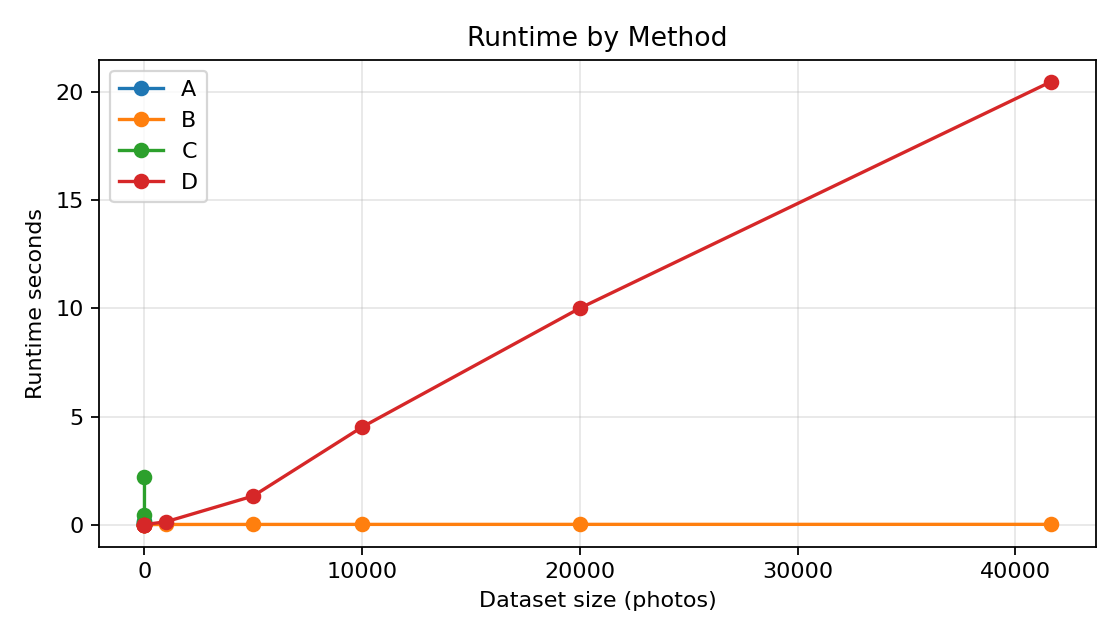
\includegraphics[width=\columnwidth]{runtime.png}
  \caption{Runtime by method and dataset size. Exact methods grow quickly and are only run on tiny samples; Method B is fastest, while Method D pays for similarity coverage.}
  \Description{Line chart of runtime by dataset size for each method.}
  \label{fig:runtime}
\end{figure}

\begin{figure}[!htbp]
  \centering
  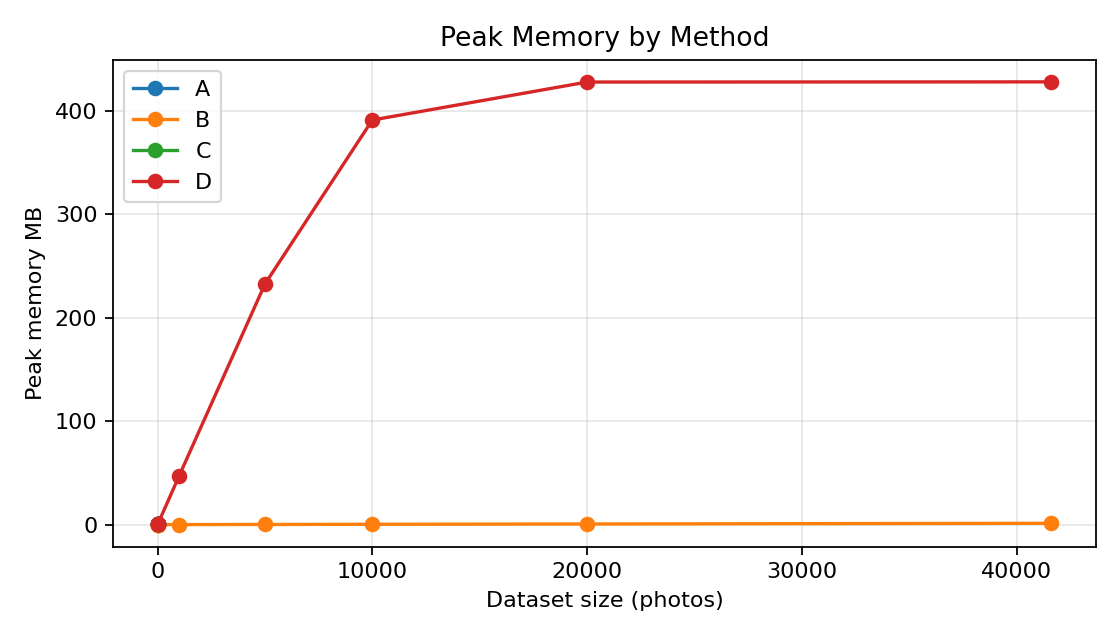
\includegraphics[width=\columnwidth]{memory.png}
  \caption{Peak measured memory by method. Method D uses more memory than IndepDF because it evaluates chunked similarity coverage.}
  \Description{Line chart of measured peak memory by dataset size for each method.}
  \label{fig:memory}
\end{figure}

\begin{table}[!htbp]
  \caption{Average small exact-comparison performance.}
  \label{tab:small-performance}
  \small
  \begin{tabular}{@{}lrr@{}}
    \toprule
    Method & Runtime (s) & Peak MB \\
    \midrule
    A & 0.064875 & 0.197561 \\
    B & 0.000342 & 0.008232 \\
    C & 0.690467 & 0.340381 \\
    D & 0.001367 & 0.440582 \\
    \bottomrule
  \end{tabular}
\end{table}

\begin{figure}[!htbp]
  \centering
  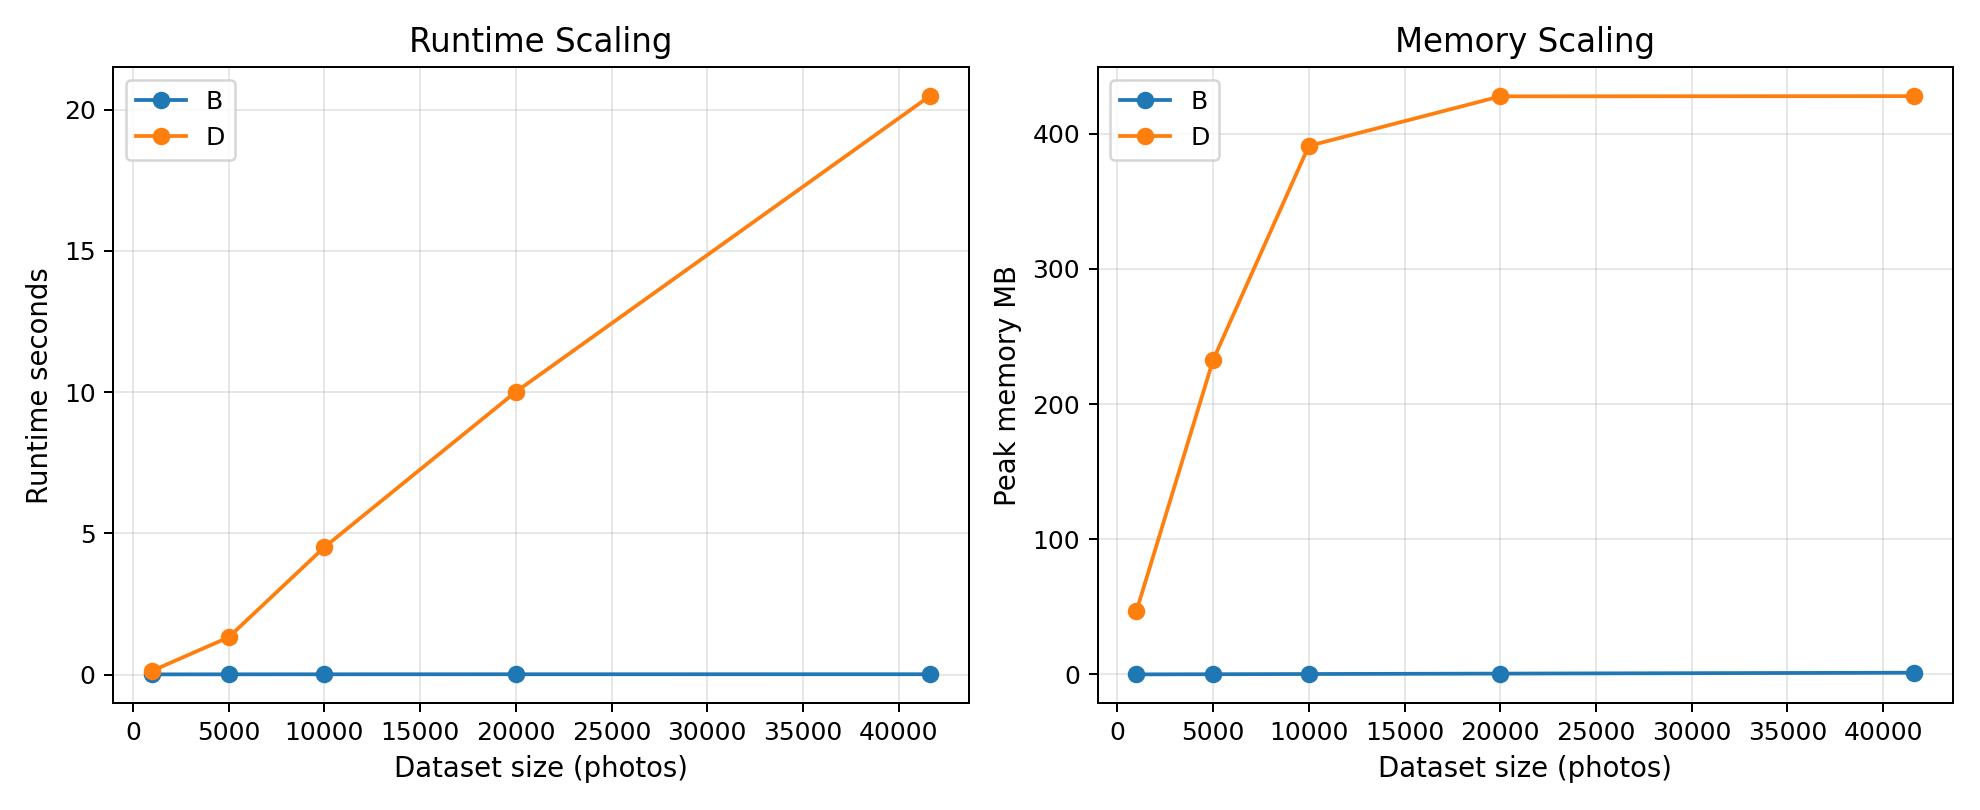
\includegraphics[width=\textwidth]{scalability.png}
  \caption{Scalability for Methods B and D across increasing query-active samples, including the full dataset. Method D remains feasible but is more expensive because its objective is embedding-coverage based.}
  \Description{Two-panel line chart showing runtime and memory scaling for Methods B and D.}
  \label{fig:scalability}
\end{figure}

Full-data exact Method A and exact Method C were skipped by design for budgets 3 and 4. Method A exceeds exhaustive-search limits, and Method C exceeds exact Shapley limits. These skipped rows are evidence of scale limits, not implementation failures.

\begin{table}[!htbp]
  \caption{Scalability batch rows for scalable methods.}
  \label{tab:scalability-rows}
  \small
  \begin{tabular}{@{}lrrr@{}}
    \toprule
    Method & Photos & Utility & Runtime (s) \\
    \midrule
    B & 1,000 & 0.302 & 0.007 \\
    B & 5,000 & 0.311 & 0.009 \\
    B & 10,000 & 0.286 & 0.011 \\
    B & 20,000 & 0.283 & 0.012 \\
    B & 41,620 & 0.283 & 0.013 \\
    D & 1,000 & 0.359 & 0.133 \\
    D & 5,000 & 0.368 & 1.322 \\
    D & 10,000 & 0.366 & 4.510 \\
    D & 20,000 & 0.371 & 10.010 \\
    D & 41,620 & 0.369 & 20.478 \\
    \bottomrule
  \end{tabular}
\end{table}

\subsection{Quality}

On the small exact comparison, Methods A and D were nearly tied under cosine-proxy utility for both $\budget=3$ and $\budget=4$, while Method B and Method C remained close. This is expected: the sampled candidate sets are small enough that exact search is meaningful, and Method D's greedy coverage often reaches the same representative structure.

\begin{table}[!htbp]
  \caption{Average small exact-comparison utility.}
  \label{tab:small-utility}
  \small
  \begin{tabular}{@{}lrrr@{}}
    \toprule
    Method & Budget & Cosine proxy & Jaccard/precision \\
    \midrule
    A & 3 & 0.612920 & 0.466651 \\
    B & 3 & 0.602152 & 0.466651 \\
    C & 3 & 0.603742 & 0.466651 \\
    D & 3 & 0.612436 & 0.466651 \\
    A & 4 & 0.696715 & 0.570696 \\
    B & 4 & 0.682184 & 0.570696 \\
    C & 4 & 0.682327 & 0.570696 \\
    D & 4 & 0.696319 & 0.570696 \\
    \bottomrule
  \end{tabular}
\end{table}

\begin{figure}[!htbp]
  \centering
  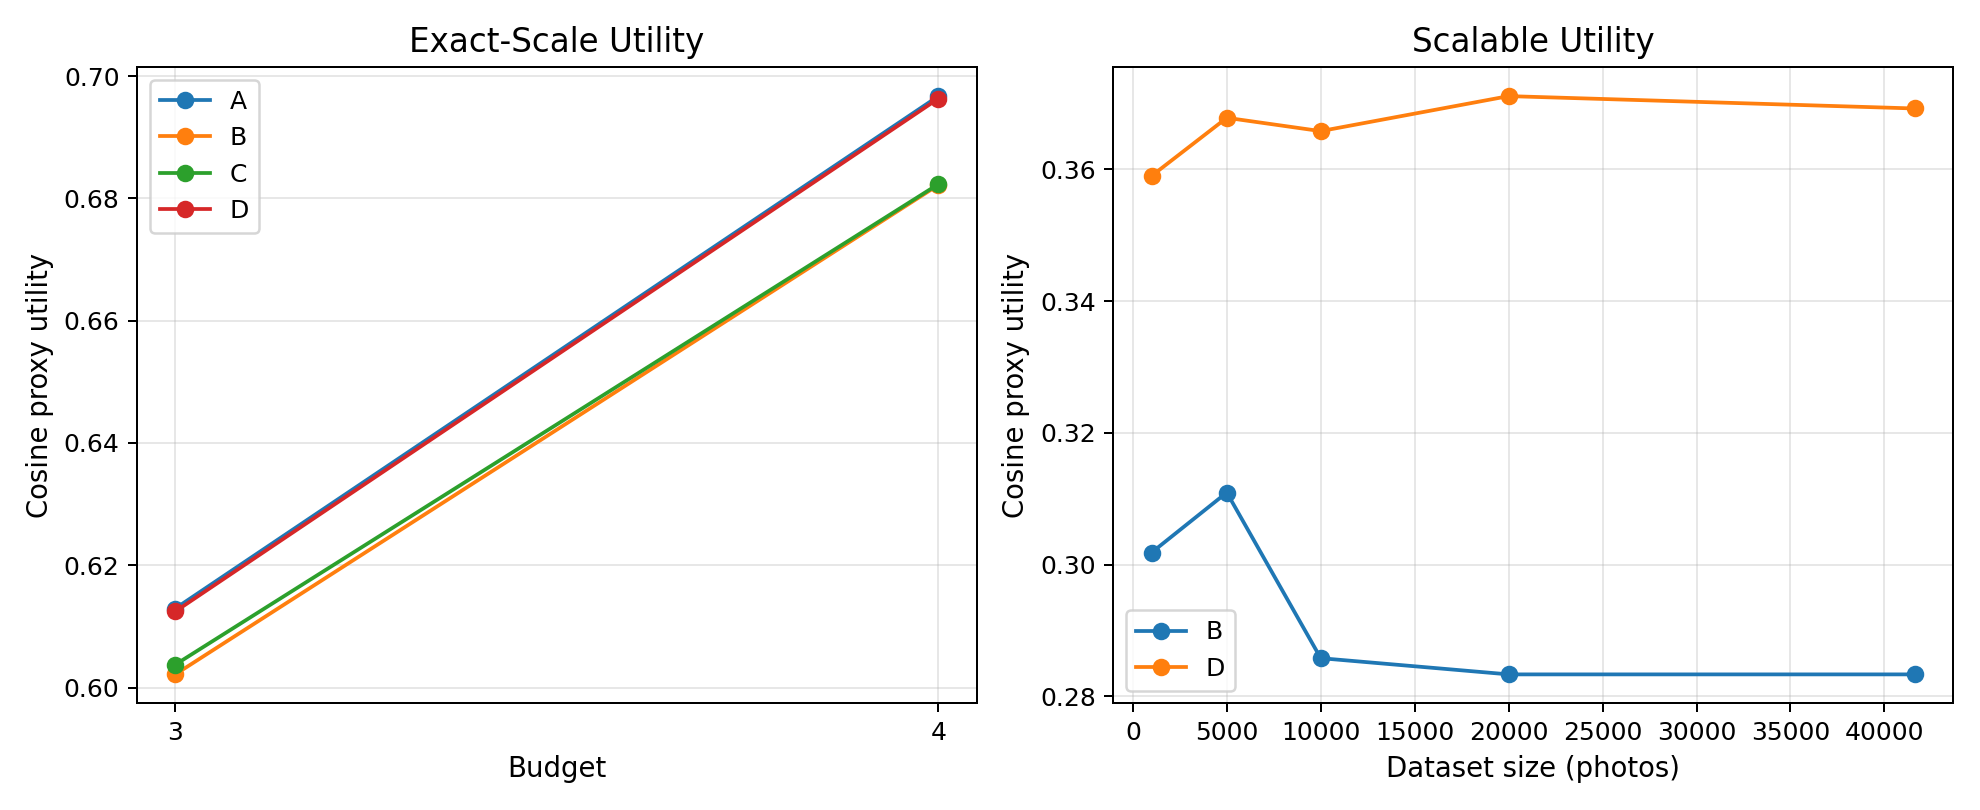
\includegraphics[width=\columnwidth]{utility.png}
  \caption{Cosine-proxy utility by method. Method D tracks the exact baseline on small samples and improves over Method B on scalable runs.}
  \Description{Two-panel line chart of cosine-proxy utility by exact-comparison budget and scalable dataset size.}
  \label{fig:utility}
\end{figure}

On larger scalable runs, Method D achieved stronger cosine-proxy utility than Method B. In the scalability batch, the mean utilities were 0.293034 for Method B and 0.366595 for Method D. In the budget-sensitivity batch, the means were 0.315245 and 0.391628, respectively.

\begin{figure}[!htbp]
  \centering
  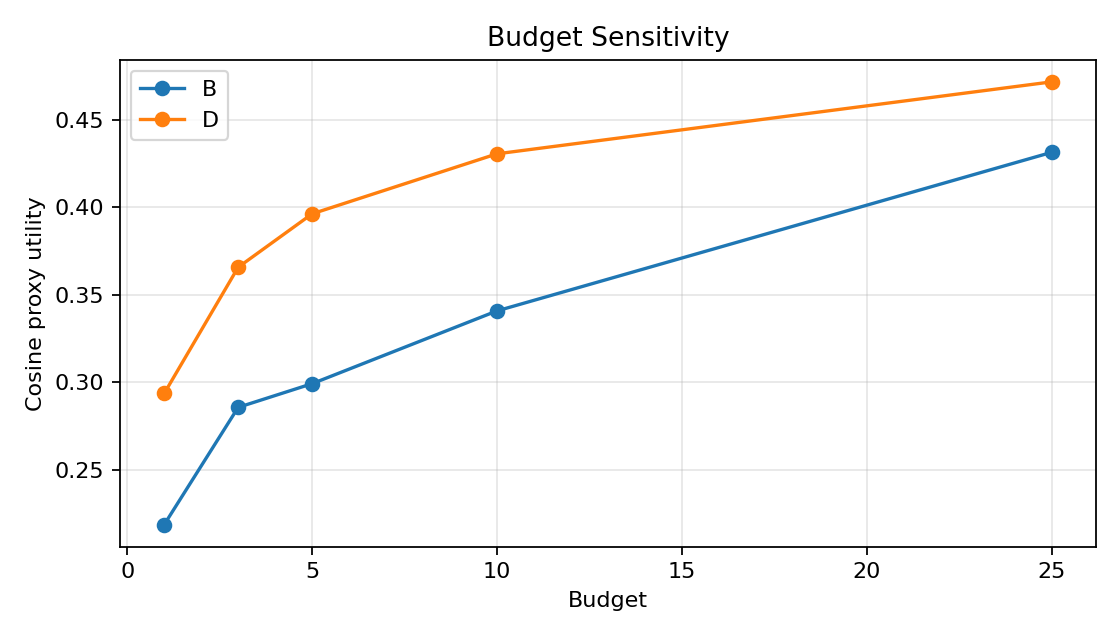
\includegraphics[width=\columnwidth]{budget_sensitivity.png}
  \caption{Budget sensitivity on a 10,000-photo query-active sample. Both scalable methods improve as the retention budget grows, with Method D preserving more embedding-level utility.}
  \Description{Line chart of cosine-proxy utility by budget for Methods B and D.}
  \label{fig:budget}
\end{figure}

The Method D ablation batch supports the combined design. Full Method D averaged 0.422695 cosine-proxy utility, coverage-only averaged 0.421382, and frequency-only averaged 0.352703. Frequency-only had higher Jaccard/precision utility but lower embedding coverage, which is consistent with its popularity-only behavior.

\begin{table}[!htbp]
  \caption{Budget sensitivity rows on the 10,000-photo sample.}
  \label{tab:budget-rows}
  \small
  \begin{tabular}{@{}lrrr@{}}
    \toprule
    Method & Budget & Utility & Runtime (s) \\
    \midrule
    B & 1 & 0.219 & 0.011 \\
    B & 3 & 0.286 & 0.011 \\
    B & 5 & 0.299 & 0.011 \\
    B & 10 & 0.341 & 0.011 \\
    B & 25 & 0.431 & 0.012 \\
    D & 1 & 0.294 & 1.712 \\
    D & 3 & 0.366 & 4.535 \\
    D & 5 & 0.396 & 7.600 \\
    D & 10 & 0.431 & 15.124 \\
    D & 25 & 0.472 & 37.721 \\
    \bottomrule
  \end{tabular}
\end{table}

\begin{table}[!htbp]
  \caption{Method D ablation means.}
  \label{tab:ablations}
  \small
  \begin{tabular}{@{}lrr@{}}
    \toprule
    Variant & Cosine proxy & Jaccard/precision \\
    \midrule
    D & 0.422695 & 0.004007 \\
    Coverage-only & 0.421382 & 0.000976 \\
    Frequency-only & 0.352703 & 0.026869 \\
    \bottomrule
  \end{tabular}
\end{table}

\begin{figure}[!htbp]
  \centering
  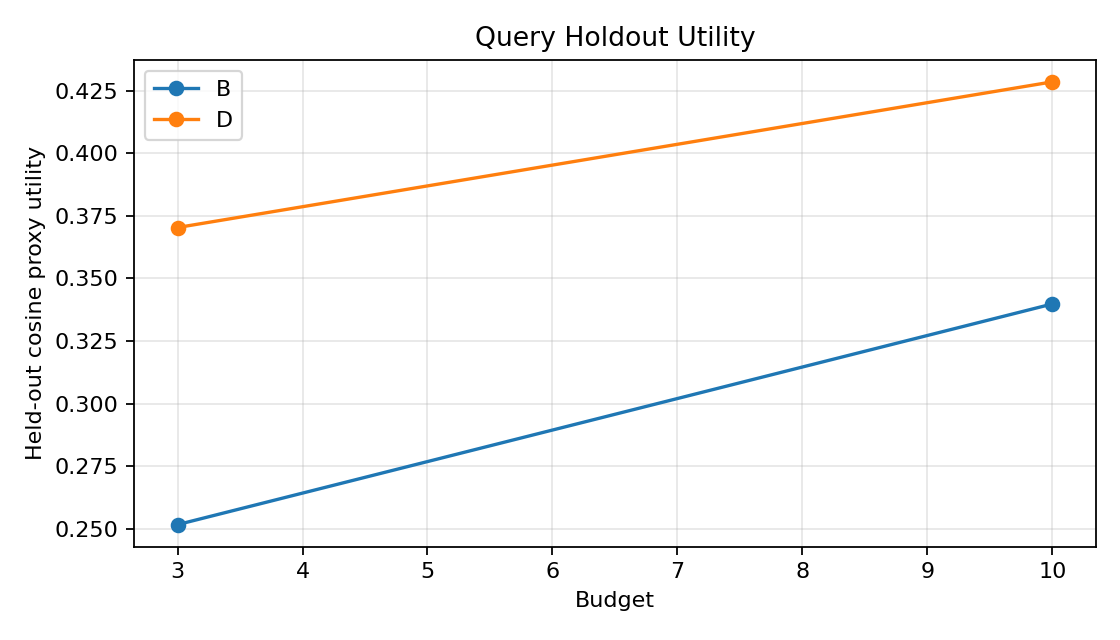
\includegraphics[width=\columnwidth]{holdout_utility.png}
  \caption{Held-out query utility for Methods B and D on a 10,000-photo query-active sample. Methods are trained on 75\% of projected query rows and evaluated on the remaining 25\%.}
  \Description{Line chart of held-out cosine-proxy utility by budget for Methods B and D.}
  \label{fig:holdout}
\end{figure}

\begin{table}[!htbp]
  \caption{Query-holdout means over three seeds.}
  \label{tab:holdout}
  \small
  \begin{tabular}{@{}lrrr@{}}
    \toprule
    Method & Budget & Held-out utility & Runtime (s) \\
    \midrule
    B & 3 & 0.251655 & 0.009 \\
    B & 10 & 0.339812 & 0.009 \\
    D & 3 & 0.370361 & 3.887 \\
    D & 10 & 0.428558 & 12.766 \\
    \bottomrule
  \end{tabular}
\end{table}

\subsection{Held-Out Query Robustness}

The query-holdout batch addresses whether the scalable methods merely fit the same query rows used for scoring. For each seed, the runner trains Method B or Method D on 75\% of the projected query rows and evaluates the selected photos on the remaining 25\%. Method D remains stronger under this split: averaged over budgets and seeds, held-out cosine-proxy utility is 0.399460 for Method D and 0.295733 for Method B. This does not prove chronological generalization, because the query log has no timestamps, but it is a useful robustness check against evaluating only on the training query rows.

\subsection{Interpreting the Metrics}

The gap between cosine-proxy utility and Jaccard/precision utility is informative. Frequency-only selection can score relatively well on Jaccard/precision because it keeps photos that historically appeared often. However, it can fail to represent visually similar alternatives. Coverage-only selection can improve embedding representativeness but may waste budget on regions that rarely matter to the query log. Method D combines the two signals, which explains why it is the strongest scalable method under the primary cosine-proxy metric.

The exact small-sample utility table also shows why no single baseline is enough. Method A is the best possible set under the cosine proxy for those samples, but it cannot scale. Method B is almost instantaneous, but it does not optimize embedding replacement. Method C is conceptually attractive, but ranking individual Shapley values does not always capture interactions between selected photos. Method D is the compromise: it is not exact, but it directly optimizes a coverage objective that reflects the assignment's search-preservation goal.

\section{Additional Observations}

\subsection{Synthetic Sanity Checks}

The synthetic batch is not meant to replace the private assignment dataset. Its role is to make the behavior of the methods easier to reason about. Synthetic clustered data creates small embedding groups with known structure, so a coverage method should prefer representatives from useful clusters rather than arbitrary frequent IDs. In that setting, Method A and Method D both reached an average cosine-proxy utility of 0.997714, while Method B averaged 0.789133. This is consistent with the intended design: when the embedding geometry has clear clusters, greedy facility location can recover the same coverage pattern as exact search on feasible instances.

On synthetic data, Method C averaged 0.371130 cosine-proxy utility. Its Jaccard/precision utility was 0.458946. This does not mean Shapley values are incorrect. It shows that exact individual contribution ranking can disagree with the best size-$B$ set under a coverage objective, especially when the selected set needs complementary representatives. This supports reporting Method C as a principled baseline rather than as the final scalable solution.

\begin{table}[!htbp]
  \caption{Synthetic sanity-check means.}
  \label{tab:synthetic}
  \small
  \begin{tabular}{@{}lrrr@{}}
    \toprule
    Method & Cosine proxy & Jaccard/precision & Runtime (s) \\
    \midrule
    A & 0.997714 & 0.382376 & 0.444359 \\
    B & 0.789133 & 0.426743 & 0.000519 \\
    C & 0.371130 & 0.458946 & 1.360460 \\
    D & 0.997714 & 0.382376 & 0.001392 \\
    \bottomrule
  \end{tabular}
\end{table}

\subsection{Exact-Scale Interpretation}

The small exact comparison is the most important bridge between correctness and scalability. It uses real data, query-active sampling, and $\budget \in \{3,4\}$, while keeping the candidate sets small enough for Methods A and C. The result that Method D nearly matches Method A is encouraging because Method D is not explicitly enumerating all subsets. Instead, it uses the same coverage intuition in a greedy form.

The identical average Jaccard/precision values within each budget in Table~\ref{tab:small-utility} are also worth noting. On these tiny query-active samples, the selected sets often preserve similar membership fractions even when the cosine-proxy choices differ. This is one reason the report emphasizes cosine-proxy utility as the primary metric for distinguishing embedding-aware behavior. The membership metric is useful, but it can be too coarse when the budget is tiny and sampled queries overlap heavily.

\subsection{Why Method D Is the Main Proposal}

Method D is not chosen because it wins every metric. It is chosen because it best matches the assignment's practical objective. The user wants to keep a small photo subset that remains useful for search. A pure frequency method may keep common photos, but it can miss visual coverage. A pure exact method gives beautiful answers on toy inputs but cannot run at assignment scale. Method D is the middle path: it uses historical query evidence to decide what matters and embedding coverage to decide what can represent it.

\section{Discussion and Comparison}

The methods show a clear cost-quality trade-off. Exact methods are valuable for small correctness and comparison settings, but they do not scale to the full dataset. IndepDF is the best choice when speed and memory dominate. Method D is the best mobile-deployment candidate when the device can afford an offline selection step and the goal is to preserve embedding-level search quality.

The main limitation is workload drift: future queries may differ from the historical queries used for weighting. Exact Methods A and C also cannot serve as full-data baselines because their complexity is too high. Finally, embedding-aware conclusions depend on cosine similarity being a meaningful replacement-quality proxy for the provided vectors.

\begin{table}[!htbp]
  \caption{Overall comparison of Methods A--D.}
  \label{tab:comparison}
  \small
  \begin{tabularx}{\textwidth}{@{}lYYYY@{}}
    \toprule
    Method & Utility behavior & Runtime/memory & Complexity & Scalability \\
    \midrule
    A & Exact cosine optimum on tiny samples & Quickly infeasible & $\mathcal{O}\!\left(\binom{m}{B}\cdot \mathrm{eval}\right)$ & Tiny only \\
    B & Query-frequency baseline; weak coverage & Fastest and lightest & Query memberships plus sorting & Full dataset \\
    C & Individual contribution estimate & Exact version expensive & Exponential coalitions & Tiny only \\
    D & Strongest scalable cosine utility & Slower and heavier than B & Greedy marginal gains & Full dataset with chunking \\
    \bottomrule
  \end{tabularx}
\end{table}

\subsection{Mobile Deployment View}

For a mobile-device scenario, selection does not need to run interactively every time a user searches. It can run as an offline maintenance job when the device is charging or when storage pressure becomes severe. Under that assumption, Method D's additional runtime is acceptable because the resulting retained subset better preserves embedding-level query utility. If the device needs an immediate answer, Method B is the safer fallback because it is simple, fast, and low-memory.

The selected subset should also be reviewed as a recommendation rather than an irreversible deletion command. The implementation solves the technical selection problem, but user trust matters: users may want to pin important personal photos regardless of query history. A production system would therefore combine Method D with user constraints such as never-delete albums, favorites, recent photos, or privacy-sensitive categories.

\subsection{Threats to Validity}

The first threat is workload drift. Historical queries may not represent future information needs, especially after travel, new events, or changes in user behavior. The second threat is embedding mismatch: if the provided vectors do not capture the semantic distinctions users care about, cosine similarity may overestimate replacement quality. The third threat is sampling bias in exact comparisons. Methods A and C are evaluated only on query-active samples small enough to be feasible, so those results validate behavior rather than full-dataset optimality. The final threat is measurement noise on runtime and memory, which can vary across local machine state. The report mitigates this by recording hardware notes and focusing on broad trends.

\subsection{Ethical and Practical Notes}

Deleting personal photos is more sensitive than deleting anonymous benchmark rows. A real phone application should not treat the selected subset as an automatic deletion order. It should expose the recommendation, explain why photos were kept or marked as low value, and allow users to protect favorites, recent memories, albums, or sensitive categories. Query-aware selection is useful because it connects retention to observed behavior, but observed behavior is not the same thing as personal importance.

Privacy also matters. Query logs can reveal habits, locations, and relationships. This project keeps all processing local and does not commit raw data. A deployed system should follow the same principle: compute weights and retained sets on-device where possible, and avoid uploading raw embeddings or query histories unless the user explicitly chooses a cloud service.

\section{Future Work}

The most direct extension is Monte Carlo Shapley estimation. Exact Shapley is impossible on the full dataset, but sampled permutations could provide an approximate importance ranking at larger scales. This would make Method C more useful as a practical baseline while preserving its game-theoretic interpretation.

A second extension is a clustering or medoid baseline. Such a method would ignore query frequency and optimize only visual representativeness. Comparing it to Method D would further isolate how much value comes from workload awareness. The current coverage-only ablation partially answers this question, but a standard clustering baseline would be easier to compare with broader data-reduction literature.

A third extension is user constraints. The current budget treats every photo as equal cost and equally deletable. A realistic mobile system would support hard constraints and weighted costs: never delete favorites, prefer recent photos, preserve at least one item per album, or account for different file sizes. Method D could incorporate such constraints by filtering candidates, adjusting costs, or using a knapsack-style greedy variant.

Finally, future experiments could evaluate robustness under chronological workload drift. The current report adds a random query-holdout split, but timestamps would allow a stronger test: training weights on earlier queries and evaluating utility on later queries. Chronological drift would better match the real question of whether historical behavior predicts future search needs.

\begin{table}[!htbp]
  \caption{Possible extensions and expected benefit.}
  \label{tab:future}
  \small
  \begin{tabularx}{\columnwidth}{@{}lX@{}}
    \toprule
    Extension & Benefit \\
    \midrule
    Monte Carlo Shapley & scalable approximation to Method C \\
    Clustering baseline & clearer visual-representativeness comparison \\
    User constraints & safer deletion recommendations for personal photos \\
    Chronological drift evaluation & stronger test of historical-query generalization \\
    File-size costs & closer match to actual storage-pressure decisions \\
    \bottomrule
  \end{tabularx}
\end{table}

\section{Reproducibility}

The repository is organized as a Python 3.12 project managed by \texttt{uv}. Raw data is intentionally ignored by git, so a clean clone requires placing \texttt{photos.csv} and \texttt{queries.csv} under \texttt{data/raw/}. The core verification commands are:
\begin{verbatim}
uv sync
uv run python scripts/validate_data.py
uv run pytest
uv run ruff check .
uv run python scripts/generate_figures.py \
  --results experiments/results \
  --output experiments/figures
\end{verbatim}
The project also includes a \texttt{Makefile} with check, full-experiment, and figure targets. Saved experiment rows are stored as tidy CSV files with diagnostics JSON artifacts and batch metadata, including Python version, platform, hardware notes, config hash, git commit, dirty flag, and data diagnostics.

\subsection{Quality Controls}

The automated test suite covers CSV parsing, ID normalization, invalid data handling, cosine similarity, utility calculations, method determinism, budget validation, exact-method skips, Method D chunking, experiment grid expansion, query-holdout evaluation, diagnostics writing, and figure generation. The final local verification command reports 62 passing tests, and Ruff reports no lint violations. These checks are not a substitute for mathematical proof, but they reduce the risk of implementation errors in the data pipeline and method comparison.

\section{Conclusion}

This project implements and evaluates all required methods for query-aware photo reduction. The final recommendation is to use Method D when the objective is high-quality offline selection for a mobile device, because it balances popularity, diversity, and embedding-level representativeness. If selection must be extremely fast or memory-constrained, Method B is the practical fallback. Methods A and C should be retained as exact or principled tiny-scale baselines, not as deployable full-dataset methods.

Method D is not a universal deletion policy. It inherits the biases of the historical query log and the embedding representation. Nevertheless, within the assignment setting it provides a strong compromise: it is faithful to the workload, explicitly uses visual similarity, and can be run on the full local dataset with documented memory guardrails. That makes it the most appropriate strategy among the implemented methods for preparing a reduced photo collection while preserving expected query usefulness.

\bibliographystyle{ACM-Reference-Format}
\bibliography{references}

\end{document}
